% Created 2021-01-12 Tue 22:46
% Intended LaTeX compiler: pdflatex
\documentclass[11pt]{article}
\usepackage[utf8]{inputenc}
\usepackage[T1]{fontenc}
\usepackage{graphicx}
\usepackage{grffile}
\usepackage{longtable}
\usepackage{wrapfig}
\usepackage{rotating}
\usepackage[normalem]{ulem}
\usepackage{amsmath}
\usepackage{textcomp}
\usepackage{amssymb}
\usepackage{capt-of}
\usepackage{hyperref}
\author{Adriel Benati de Melo}
\date{12 de Janeiro}
\title{Lista de Exercícios 2}
\hypersetup{
 pdfauthor={Adriel Benati de Melo},
 pdftitle={Lista de Exercícios 2},
 pdfkeywords={},
 pdfsubject={},
 pdfcreator={Emacs 27.1 (Org mode 9.4.4)}, 
 pdflang={English}}
\begin{document}

\maketitle

\section*{4)}
\label{sec:orgcd07a13}

\subsection*{a) e b)}
\label{sec:org6e8c663}

Tomado o conjunto (7, 8, 6, 10, 5, 9, 4, 12, 7, 8), tem-se que:

\begin{verbatim}
Média do conjunto =  8
Desvio padrão do conjunto = 2
\end{verbatim}

\section*{13)}
\label{sec:orgbeb687d}

Os extremos são 1 e 12, os quartis 2 e 6, e a mediana 4.

\section*{19)}
\label{sec:orgb2fd997}

\subsection*{a)}
\label{sec:org1ca2407}

\begin{verbatim}
dist <- c(1.8, 2.5, 0.4, 1.9, 4.4, 2.2, 3.5, 0.2, 0.9, 1.4, 1.1,
1.7, 1.2, 2.3, 1.9, 0.8, 1.5, 1.7, 1.4, 2.1, 3.2, 15.1, 2.1, 1.4,
0.5, 0.9, 1.7, 0.5, 0.8, 3.7, 1.4, 1.8, 2.0, 1.1, 1.0, 0.8)

stem(dist, scale = 2)
\end{verbatim}

\begin{verbatim}

The decimal point is at the |

 0 | 245588899
 1 | 0112444457778899
 2 | 011235
 3 | 257
 4 | 4
 5 | 
 6 | 
 7 | 
 8 | 
 9 | 
10 | 
11 | 
12 | 
13 | 
14 | 
15 | 1

\end{verbatim}

\subsection*{b)}
\label{sec:org09a4082}

\begin{verbatim}
           aaa  bbb
Min.     0.200 0.40
1st Qu.  0.975 1.60
Median   1.600 2.80
Mean     2.025 3.56
3rd Qu.  2.100 4.20
Max.    15.100 8.80
\end{verbatim}

\subsection*{c)}
\label{sec:org367c05f}

\begin{center}
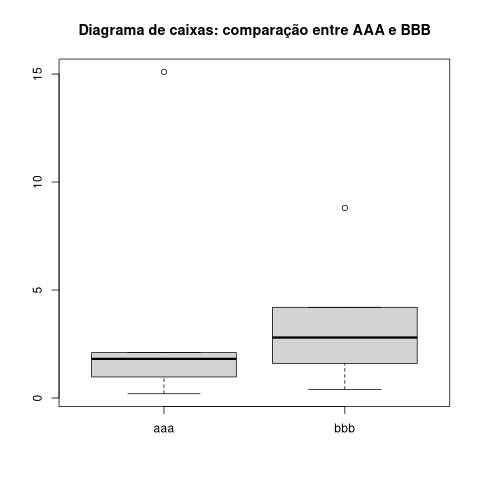
\includegraphics[width=.9\linewidth]{boxplot.png}
\end{center}
\end{document}